% Options for packages loaded elsewhere
\PassOptionsToPackage{unicode}{hyperref}
\PassOptionsToPackage{hyphens}{url}
%
\documentclass[
]{article}
\usepackage{lmodern}
\usepackage{amssymb,amsmath}
\usepackage{ifxetex,ifluatex}
\ifnum 0\ifxetex 1\fi\ifluatex 1\fi=0 % if pdftex
  \usepackage[T1]{fontenc}
  \usepackage[utf8]{inputenc}
  \usepackage{textcomp} % provide euro and other symbols
\else % if luatex or xetex
  \usepackage{unicode-math}
  \defaultfontfeatures{Scale=MatchLowercase}
  \defaultfontfeatures[\rmfamily]{Ligatures=TeX,Scale=1}
\fi
% Use upquote if available, for straight quotes in verbatim environments
\IfFileExists{upquote.sty}{\usepackage{upquote}}{}
\IfFileExists{microtype.sty}{% use microtype if available
  \usepackage[]{microtype}
  \UseMicrotypeSet[protrusion]{basicmath} % disable protrusion for tt fonts
}{}
\makeatletter
\@ifundefined{KOMAClassName}{% if non-KOMA class
  \IfFileExists{parskip.sty}{%
    \usepackage{parskip}
  }{% else
    \setlength{\parindent}{0pt}
    \setlength{\parskip}{6pt plus 2pt minus 1pt}}
}{% if KOMA class
  \KOMAoptions{parskip=half}}
\makeatother
\usepackage{xcolor}
\IfFileExists{xurl.sty}{\usepackage{xurl}}{} % add URL line breaks if available
\IfFileExists{bookmark.sty}{\usepackage{bookmark}}{\usepackage{hyperref}}
\hypersetup{
  pdftitle={Scenario analysis for an outbreak of COVID-19 on a university campus},
  pdfauthor={John M. Drake},
  pdfkeywords={COVID-19, coronavirus, non-pharmaceutical interventions, SARS-CoV-2},
  hidelinks,
  pdfcreator={LaTeX via pandoc}}
\urlstyle{same} % disable monospaced font for URLs
\usepackage[margin=1in]{geometry}
\usepackage{graphicx,grffile}
\makeatletter
\def\maxwidth{\ifdim\Gin@nat@width>\linewidth\linewidth\else\Gin@nat@width\fi}
\def\maxheight{\ifdim\Gin@nat@height>\textheight\textheight\else\Gin@nat@height\fi}
\makeatother
% Scale images if necessary, so that they will not overflow the page
% margins by default, and it is still possible to overwrite the defaults
% using explicit options in \includegraphics[width, height, ...]{}
\setkeys{Gin}{width=\maxwidth,height=\maxheight,keepaspectratio}
% Set default figure placement to htbp
\makeatletter
\def\fps@figure{htbp}
\makeatother
\setlength{\emergencystretch}{3em} % prevent overfull lines
\providecommand{\tightlist}{%
  \setlength{\itemsep}{0pt}\setlength{\parskip}{0pt}}
\setcounter{secnumdepth}{-\maxdimen} % remove section numbering
\usepackage{amsmath,epsfig}
\usepackage{amssymb,amsthm}
\usepackage[all]{xy}
\usepackage{xcolor}
\usepackage{mathtools}
\usepackage{mathrsfs}
\geometry{margin=1in}

% Header and Footer
\usepackage{fancyhdr}
\pagestyle{fancy}
\fancypagestyle{plain}{\pagestyle{fancy}}
\fancyhf{}
\fancyhead[CO,CE]{Working paper}
\fancyfoot[LE,RO]{\thepage}

\title{Scenario analysis for an outbreak of COVID-19 on a university campus}
\author{John M. Drake}
\date{August 15, 2020}

\begin{document}
\maketitle
\begin{abstract}
Significant uncertanties remain concerning the opening of college and
university campuses in the United States due to COVID-19. We assembled
quantitative empirical information about several processes likely to
affect the transmission of SARS-CoV-2 within institutions of higher
education. Preliminary results suggest that campuses should anticipate
explosive localized outbreaks and be prepared for significant levels of
transmission associated with the congregation of students. We identify
off-campus student-student interactions to be the arena of intervention
with the greatest opportunity for significant reductions in
transmission.
\end{abstract}

\hypertarget{executive-summary}{%
\section{Executive Summary}\label{executive-summary}}

Numerous American colleges and universities are planning to reopen for
fall instruction. It is widely anticipated that the congregation of
students will lead to new outbreaks of COVID-19. Institutions have
accordingly adopted policies and procedures designed to limit the spread
of SARS-CoV-2, but the effectiveness of these procedures is currently
unknown. Models are a useful tool for planning and scenario analysis in
the absence of empirical information. However, there are several
information gaps that make modeling of transmission within a university
community particularly difficult, including how population segmentation
(i.e.~faculty, students, and staff) affects transmission; mixing rates
among these segments; efficacy of generalized interventions such as
wearing face masks, reducing student density, and installing infection
barriers; and the extent of airborne, droplet, and surface contact
transmission.

As with all current models, the following analysis is subject to these
limitations. We are not, however, completely ignorant about the
qualitative and quantitative properties of transmission by symptomatic
and asymptomatic persons, the effectiveness of interventions, and
usefulness of testing to identify asymptomatic carriers. In particular,
compartmental models have been shown to be robust to a wide range of
structural uncertainties and effectively represent the sometimes
counter-intuitive properties of epidemics. Using the State of Georgia as
an example, we modeled an outbreak of COVID-19 for a typical large state
university with a population of 50,000. Key findings of our analysis
include:

\begin{itemize}
\tightlist
\item
  \textbf{Campus-based interventions are unlikely to prevent an epidemic
  of COVID-19 within the campus community.}
\item
  \textbf{From 210 to 1618 imported infections may be expected with the
  arrival of students for Fall 2020.}
\item
  \textbf{To reduce the basic reproduction number (\(\mathcal{R}_{0}\))
  to less than one, a testing program would need to administer
  approximately 6,181 tests per day at typical levels of protection
  (face masks, social distancing, etc.)}
\item
  \textbf{Effective containment of COVID-19 at large institutions of
  higher education will require the widespread adoption of behavioral
  practices among students that reduce transmission of SARS-CoV-2
  off-campus.}
\end{itemize}

\hypertarget{model}{%
\section{Model}\label{model}}

We developed a compartmental model of COVID-19 transmission on a
university campus that includes asymptomatic transmission and accounts
for surveillance testing and case isolation as well as generalized
interventions. Individual persons are classified as Susceptible (\(S\)),
Latent or presymptomatic (\(L\)), Asymptomatic (\(A\)), symptomatic and
Infectious (\(I\)), or Removed through recovery or isolation (\(R\))
(Fig. \ref{fig:university_model}).

\begin{figure}

{\centering 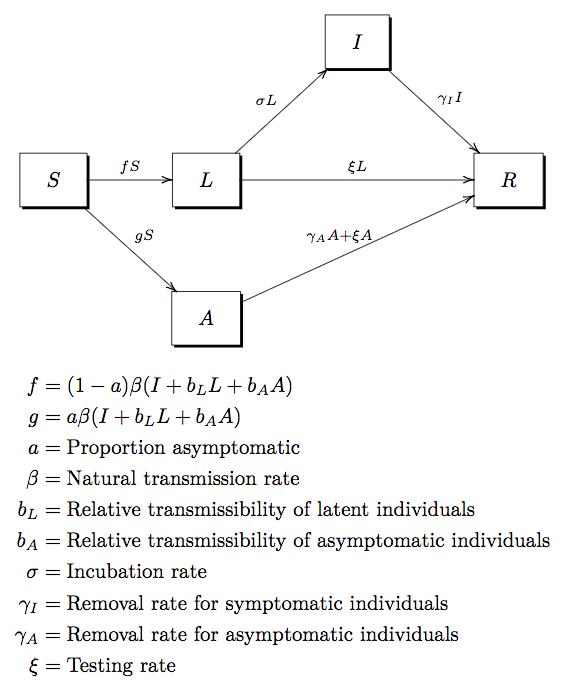
\includegraphics[width=0.7\linewidth]{university_SLAIR} 

}

\caption{\label{fig:university_model}Compartmental model for SARS-CoV-2 on a university campus.}\label{fig:unnamed-chunk-1}
\end{figure}

The system of ordinary differential equations for this model is
\begin{align*}
\dot{S} & =-\beta\left(I+b_{L}L+b_{A}A\right)S,\\
\dot{L} & =\left(1-a\right)\beta\left(I+b_{L}L+b_{A}A\right)S-\left(\sigma+\xi\right)L,\\
\dot{A} & =a\beta\left(I+b_{L}L+b_{A}A\right)S-\left(\gamma_{A}+\xi\right)A,\\
\dot{I} & =\sigma L-\gamma_{I}I,\\
\dot{R} & =\gamma_{I}I+\gamma_{A}A+\xi L+\xi A.
\end{align*} We simplify the notation by defining \begin{align*}
f & =\left(1-a\right)\beta\left(I+b_{L}L+b_{A}A\right), \text{and}\\
g & =a\beta\left(I+b_{L}L+b_{A}A\right).
\end{align*} Let \(N=S+L+A+I+R\) represent the total population. Then
\(\dot{N}=0\). Thus the disease-free equilibrium is given by
\(S_{0}=N_{0}=N\left(0\right)\), with all other state variables equal to
zero.

The infectious compartments are represented by \(L\), \(A\), and \(I\).
The basic reproduction number is: \[
\mathcal{R}_{0}=\beta N_{0}\left(1-a\right)\left[b_{L}\frac{1}{\left(\sigma+\xi\right)}+\frac{1}{\gamma_{I}}\left(\frac{\sigma}{\sigma+\xi}\right)\right]+\beta N_{0}ab_{A}\left(\frac{1}{\gamma_{A}+\xi}\right).
\]

\hypertarget{implementation}{%
\subsubsection{Implementation}\label{implementation}}

Here we parameterize our model for a large state university, using the
demographics and health statistics of the state of Georgia as an
example. We assume the university will use testing and case isolation in
combination with generalized interventions to reduce transmission. We
use our model to examine scenarios for the possibility of outbreak
within the university community.

The essential disease parameters apply to any population. We assume an
incubation period of 4 days, giving \(\sigma=\) 0.25
({[}\protect\hyperlink{ref-Zhang2020-ih}{1}{]},
{[}\protect\hyperlink{ref-Li2020-hc}{2}{]},
{[}\protect\hyperlink{ref-Lauer2020-mr}{3}{]}). We assume that
incubating infections are 30.0\% as contagious as symptomatic infections
so \(b_{L}=\) 0.3. Asymptomatic infections are assumed to be 50.0\% as
contagious as symptomatic infections, so \(b_{A} =\) 0.5
{[}\protect\hyperlink{ref-Li2020-hc}{2}{]}.

The contagious period of asymptomatic individuals is assumed to be 14
days, giving \(\gamma_A=\) 0.0714286
({[}\protect\hyperlink{ref-Long2020-ny}{4}{]},
{[}\protect\hyperlink{ref-Oran2020-aq}{5}{]}). We set recovery rate for
symptomatic cases to \(\gamma_I=\) 1, indicating that symptomatic
infectious individuals are assumed removed from the population within
one day because of testing or self-reporting and subsequent isolation.

University population, \(N_0\), and testing rate, \(\xi\), are specific
to the university. We use a total university population of 50,000,
40,000 of which are students (80.0\%), and 10,000 or which are staff
(20.0\%).

We assume a program of randomized surveillance (300 tests per day) with
isolation of symptomatic cases (cases detected as a result of testing or
reporting). Thus, 300 \(\div\) 50,000 \(\approx\) 0.6\% of the
population will be tested daily, represented in the model by \(\xi=\)
0.006.

The transmission rate \(\beta\) within the university population is
estimated from the expression for \(\mathcal{R}_{0}\), by setting
\(\xi\) to 0 and solving for \(\beta\),

\[
\beta= \frac{\mathcal{R}_{0}}{N_{0}\left(1-a\right)\left[\frac{b_{L}}{\sigma}+\frac{1}{\gamma_{I}}\right]+\left(\frac{N_{0}ab_{A}}{\gamma_{A}}\right)}.
\]

Our notional case assumes the basic reproduction number in the absence
of a testing program is \(\mathcal{R}_{0}= 3.0\)
{[}\protect\hyperlink{ref-Park2020-vl}{6}{]}, although we relax this
assumption in sensitivity analysis. For the notional case, the estimated
transmission rate is \(\beta =\) \ensuremath{1.3761468\times 10^{-5}}.

\hypertarget{interventions-compliance}{%
\subsubsection{Interventions \&
Compliance}\label{interventions-compliance}}

The most challenging problem (and most speculative part of this
analysis) is anticipating the effectiveness of a university's
generalized interventions like reducing student and staff density,
requiring students and staff to wear masks, and improving workplace
hygiene through cleaning and disinfection, provision of hand sanitizer,
and minimizing the use of shared resources like office supplies,
refrigerators, and photocopiers. We do not currently have a reliable
method to estimate the effectiveness of these interventions empirically,
and instead estimate effectiveness using a conceptual model that
considers transmission across three basic interaction types by three
primary transmission routes. How the three transmission routes
contribute to overall transmission is not precisely known. We assume:
(1) Aerosolized ``airborne'' transmission = 20.0\%, (2) Droplet
transmission = 40.0\%, and (3) Contact surfaces = 40.0\%. Masks reduce
(1) and (2) by about 65.0\% and ``healthy workplace'' practices reduce
(3) by about 75.0\% ({[}\protect\hyperlink{ref-Offeddu2017-ae}{7}{]},
{[}\protect\hyperlink{ref-Bowen2010-ht}{8}{]},
{[}\protect\hyperlink{ref-Reynolds2016-oy}{9}{]}). Thus, with full
compliance, interventions might reduce transmission by 0.2 \(\times\)
0.65 + 0.4 \(\times\) 0.65 + 0.4 \(\times\) 0.75 \(=\) 0.69.

We suppose compliance is based on transmission type. The three
transmission types are: (1) student-student, (2) student-staff, and (3)
staff-staff. For \(m=\) 40,000 students and \(n=\) 10,000 staff, there
are \(m^2-m \approx 1.6 \text{ billion}\) possible student-student
interactions, \(m \times n \approx 400 \text{ million}\) student-staff
interactions, and \(n^2-n \approx 100 \text{ million}\) staff-staff
interactions for a total of 2,099,950,000 possible interactions.
Translated into percentages, student-student interactions are 76.2\% of
the total, student-staff interactions are 19.0\% of the total, and
staff-staff interactions are 4.8\% of the total. We assume that mask and
healthy workplace interventions have their estimated effectiveness at
all times at which people are engaged in on-campus activities and that
all student-staff and staff-staff interactions are on-campus activities,
but that off-campus student-student interactions are non-compliant. We
further assume that students spend 15 hours per week engaged in on
campus activities, \(7 \times 8 =\) 56 hours per week sleeping, and the
remaining \(168~-\) 15 \(-\) 56 \(=\) 97 hours per week engaged in off
campus activities. Thus, we estimate that 15 \(/(\) 15 \(+\) 97 \()=\)
13.4\% of student-student interactions are compliant. Turning all of
this into a weighted average, we assume that the total reduction in
transmission due to generalized interventions will be 0.762 \(\times\)
0.134 \(\times\) 0.69 \(+\) 0.19 \(\times\) 1 \(\times\) 0.69 \(+\)
0.048 \(\times\) 1 \(\times\) 0.69 \(=\) 23.5\%. We do not attempt to
separately account for reduction in transmission due to some staff or
students performing work or attending class exclusively on-line.

With these parameters, we obtain \(\mathcal{R}_{0}=\) 2.81 for the model
with testing but no interventions and \(\mathcal{R}_{0}=\) 2.15 for the
model with testing and interventions. \textbf{We therefore conclude that
campus-based interventions are unlikely to prevent an epidemic of
COVID-19 within a large state university community without additional
measures.}

\hypertarget{initial-condition}{%
\subsubsection{Initial condition}\label{initial-condition}}

Solutions to the equations were obtained using the R package
\texttt{pomp} {[}\protect\hyperlink{ref-King2016-ra}{10}{]}. Simulating
the model forward in time requires initializing with an assumed number
of students incubating an active infection upon arrival to campus. We
assume that these are drawn randomly from within the state. For Georgia,
we observe that the 7-day moving average number of reported cases has
fluctuated around 3500 since mid-July. To infer the number of active
infections in the state requires that we correct this number for
under-reporting of symptomatic cases, correct for the incubation period,
and correct for the fraction of cases that never become symptomatic.

Our first correction is made by assuming that at least 25.0\% of
symptomatic cases are reported and at most 100\% are reported. This
yields 3,500 to 14,000 symptomatic, reportable cases per day. On
average, it takes 3-5 days for an infection to become symptomatic. In
addition, there is an approximately 4-day post-symptomatic infectious
period {[}\protect\hyperlink{ref-He2020-pq}{11}{]}. Thus, there are
between 3,500 \(\times~(\) 3 \(+\) 4 \() =\) 24,500 and 14,000
\(\times~(\) 5 \(+\) 4 \() =\) 126,000 active COVID cases in Georgia.
The symptomatic rate is believed to be between 40.0\% and 60.0\%
({[}\protect\hyperlink{ref-Pollan2020-xb}{12}{]},
{[}\protect\hyperlink{ref-Oran2020-aq}{5}{]},
{[}\protect\hyperlink{ref-Mizumoto2020-qc}{13}{]}) yielding a minimum
current number of infections in Georgia of 24,500 \(\div\) 0.6 \(=\)
40,833 and a maximum current number of infections of 126,000 \(\div\)
0.4 \(=\) 315,000. Georgia has an approximate population of 10,456,145
persons yielding a current prevalence of 0.39\% to 3.01\%. It is well
known that young adults are disproportionately likely to be infected.
The Georgia Department of Public Health has reported that between July
16 and August 11 approximately 22.3\% of total cases in the state were
persons aged 18 to 29. The US Census data table SC-EST2018-AGESEX-CIV
``Annual Estimates of the Civilian Population by Single Year of Age and
Sex for the United States and States: April 1, 2010 to July 1, 2018''
reports that 1,737,053 out of 10,456,145 (16.6\%) Georgia residents are
in this age band suggesting that college-aged residents in that state
are 0.223 \(/\) 0.1661275 \(-1=\) 34.2\% more likely to be infected than
average, leading to a statewide age-specific range for the estimated
prevalence of 0.52\% to 4.04\%. Multiplying these prevalence estimates
by the 40,000 student population of the university suggests that
\textbf{210 to 1618 imported infections may be expected with the arrival
of students for Fall 2020.}

We assume a certain number of individuals in the university population
will have already recovered from infection prior to the start of the
Fall semester. Asuming the number of reported cases in the university
prior to the Fall semester is 450, and correcting for under-reporting,
we estimate that between 450 \(\div\) 1 and 450 \(\div\) 0.25
individuals have survived an infection and/or been isolated and have
moved into the \(R\) class.

\hypertarget{what-is-the-probability-that-a-person-in-a-given-class-is-infected}{%
\subsubsection{What is the probability that a person in a given class is
infected?}\label{what-is-the-probability-that-a-person-in-a-given-class-is-infected}}

The preceding calculations suggest that the initial prevalence is
probably between 0.52\% and 4.04\%. We represent these quantities by the
letter \(p\), i.e.~\(p_{\text{low}} =\) 0.0052 and \(p_{\text{high}} =\)
0.0404. If these cases are randomly distributed among the student
population, the probability that any given person is \emph{not} infected
is \((1-p)\). Thus, the probability that \emph{one or more} students in
a class of size \(n\) are infected is \(1-(1-p)^n\). This formula is
plotted below for \(p_{\text{low}}\) and \(p_{\text{high}}\). Of course,
\(p\) will change over the course of the semester depending on how much
transmission occurs. Further insight is obtained by solving
\(1-(1-p)^n=0.5\) to obtain \(n=\frac{\log 0.5}{\log (1-p)}\). This is
the class size at which the class is more likely than not to include an
infected person. Using the upper bound, \(p_{\text{high}} =\) 0.0404, we
find that classes of 17 or more persons are more likely than not to
include an infected person. Using the lower bound, \(p_{\text{low}} =\)
0.0052, we find that classes of 132 or more persons are more likely than
not to include an infected person.

\begin{figure}

{\centering \includegraphics[width=0.7\linewidth]{manuscript_files/figure-latex/class-prob-1} 

}

\caption{\label{fig:class-size}Probability that a class contains an infected person as a function of class size. The size of the class is shown on the x-axis with lower bound (blue) and upper bound (red).}\label{fig:class-prob}
\end{figure}

\hypertarget{simulated-outbreak}{%
\subsubsection{Simulated outbreak}\label{simulated-outbreak}}

For illustration, we simulated outbreaks with and without generalized
interventions. In both cases, we assume testing of 300 asymptomatic
persons per day. Fig. \ref{fig:scenario-university} shows the epidemic
curve, i.e.~daily cases over time. Fig. \ref{fig:scenario-university-2}
shows the total outbreak size, i.e.~cumulative cases over time. These
results show that a major outbreak affecting \textgreater30,000 persons
is the most likely outcome of reopening campus under the assumed
conditions.

\begin{figure}

{\centering \includegraphics[width=0.7\linewidth]{manuscript_files/figure-latex/stochastic-university-1} 

}

\caption{\label{fig:scenario-university}Scenario analysis for an outbreak of COVID-19 on a university campus: Cases per day.}\label{fig:stochastic-university}
\end{figure}

\begin{figure}

{\centering \includegraphics[width=0.7\linewidth]{manuscript_files/figure-latex/stochastic-university-2-1} 

}

\caption{\label{fig:scenario-university-2}Scenario analysis for an outbreak of COVID-19 on a university campus: Cumulative cases over time.}\label{fig:stochastic-university-2}
\end{figure}

\hypertarget{what-test-frequency-is-required-to-bring-r_0-to-less-than-one}{%
\subsubsection{\texorpdfstring{What test frequency is required to bring
\(R_0\) to less than
one?}{What test frequency is required to bring R\_0 to less than one?}}\label{what-test-frequency-is-required-to-bring-r_0-to-less-than-one}}

The testing rate, \(\xi\), is an important parameter which can be
modified by policy. The probability of an outbreak, represented by the
basic reproduction number, can be reduced by increasing the testing rate
above a certain critical threshold, which we call the critical testing
rate, \(\xi_c\). To derive this value, where \(\mathcal{R}_{0}=1\), we
first define the following partial reproduction numbers without control:
\begin{align*}
\mathcal{R}_{L0} & =\beta S_{0}\left(1-a\right)b_{L}\frac{1}{\sigma},\\
\mathcal{R}_{I0} & =\beta S_{0}\left(1-a\right)\frac{1}{\gamma_{I}},\\
\mathcal{R}_{A0} & =\beta S_{0}ab_{A}\frac{1}{\gamma_{A}},\\
\mathcal{R}_{0} & =\mathcal{R}_{L0}+\mathcal{R}_{I0}+\mathcal{R}_{A0}.
\end{align*}

Then, the critical testing rate, is found to be \[
\xi_{c}=-\frac{1}{2}\left[\sigma\left(1-\mathcal{R}_{0}+\mathcal{R}_{A0}\right)+\gamma_{A}\left(1-\mathcal{R}_{A0}\right)\right]+\frac{1}{2}\sqrt{\left[\sigma\left(1-\mathcal{R}_{0}+\mathcal{R}_{A0}\right)+\gamma_{A}\left(1-\mathcal{R}_{A0}\right)\right]^{2}+4\sigma\gamma_{A}\left(\mathcal{R}_{0}-1\right)}.
\]

We use this formula to find the level of testing that would be required
to reduce the effective reproduction number to less than one as a
function of the effectiveness of generalized interventions (Fig.
\ref{fig:critical-xi}).

\begin{figure}

{\centering \includegraphics[width=0.7\linewidth]{manuscript_files/figure-latex/critical-xi-1} 

}

\caption{\label{fig:critical-xi}Daily number of tests required to reduce $R_0$ to less than one as a function of the effectiveness of interventions (black line). Achieving containment requires a combination of testing and intervention effectiveness above this line. Horizontal dashed line shows the size of the modeled testing program (300 tests per day). Vertical dashed line shows estimated effectiveness of on-campus transmission interventions.}\label{fig:critical-xi}
\end{figure}

\textbf{With no generalized interventions, the critical testing rate is
\(\xi_c =\) 0.2 (equivalent to 9,986 tests per day) and with generalized
interventions it is \(\xi_c^\prime =\) 0.124 (equivalent to 6,181 tests
per day).}

Uncertainty in the model parameters affects our confidence in these
estimates. To understand the effects of such variation, we performed a
sensitivity analysis of the critical testing rate. We measure
sensitivity with partial rank correlation coefficients (PRCC) because
these indices are independent of the relative magnitudes of the
parameter values.

To isolate the effect of uncertainty in epidemiological parameters on
the critical testing rate, we varied the transmission parameter
\(\beta\) so that \(\mathcal{R}_0\) ranged from \(\mathcal{R}_0=2\)
(optimistic) to \(\mathcal{R}_0=4\) (pessimistic) and varied the
remaining epidemiological parameters by +/- \(15.0%
\)\%. This was accomplished by Latin Hypercube sampling from uniform
distributions representing the range of their possible values as
follows:

\(a\sim \operatorname{Uniform}(\) 0.4 \(,\) 0.6 \()\),\\
\(b_L\sim \operatorname{Uniform}(\) 0.255 \(,\) 0.345 \()\),\\
\(b_A\sim \operatorname{Uniform}(\) 0.425 \(,\) 0.575 \()\),\\
\(\gamma_I\sim \operatorname{Uniform}(\) 0.85 \(,\) 1.15 \()\),\\
\(\gamma_A\sim \operatorname{Uniform}(~\frac{17}{280},\frac{23}{280}~)\),\\
\(\sigma\sim \operatorname{Uniform}(\) 0.2 \(,\) 0.33 \()\), and\\
\(S_0\sim \operatorname{Uniform}(\) 47,662 \(,\) 49,070 \()\).

Absent strong empirical evidence for the range of these values, the
parameters \(b_L\), \(b_A\), \(\gamma_I\), and \(\gamma_A\) are assumed
to vary by 15.0\% from their baseline values.

We performed Latin Hypercube sampling with \(500\) samples to
efficiently explore the effects of varying the parameter values on the
critical testing rate (Fig. \ref{fig:xi-sensitivity}). In the absence of
generalized interventions, the critical testing rate always exceeded
\(0.068\) per person per day, providing a lower bound of roughly
\(0.068 \times\) 50,000 \(\approx\) 3,400 individuals tested daily. When
generalized interventions are incorporated, the lower bound is then
roughly \(0.034 \times\) 50,000 \(\approx\) 1,700 individuals tested
daily.

\begin{figure}

{\centering \includegraphics[width=0.7\linewidth]{manuscript_files/figure-latex/xi-sensitivity-1} 

}

\caption{\label{fig:xi-sensitivity}Uncertainty in the critical testing rate from a Latin Hypercube Sample of the model parameters. Blue bars show critical testing rates when generalized interventions are used. Red bars show critical testing rates without generalized interventions.}\label{fig:xi-sensitivity}
\end{figure}

All parameters considered were significantly correlated to the critical
testing rate. The basic reproduction number (\(\mathcal{R}_0\)) was most
strongly correlated to the critical testing rate (PRCC value of
\(0.99\), with or without generalized interventions) while the initial
number of susceptible individuals was among the two least correlated
(PRCC value of \(0.30\), \(0.29\) with generalized interventions).

We infer that reducing the initial number of susceptible individuals on
campus would not have a significant effect on the ability for a reduced
rate of testing to control an epidemic. However, reducing the
susceptible population should have an impact on the cumulative number of
cases and daily new cases.

We also explored the effects of varying the parameter values on the
effective reproduction number \(\mathcal{R}_\text{eff}\), assuming that
the testing rate is \(\xi = 0.006\), with and without generalized
interventions (Fig. \ref{fig:re-sensitivity}). In the absence of
generalized interventions, \(\mathcal{R}_\text{eff}\) always exceeded
\(1.765\). When generalized interventions are incorporated, the lower
bound is then roughly \(1.351\). In either case,
\(\mathcal{R}_\text{eff}\) exceeds the critical threshold of one.

\begin{figure}

{\centering \includegraphics[width=0.7\linewidth]{manuscript_files/figure-latex/re-sensitivity-1} 

}

\caption{\label{fig:re-sensitivity}Uncertainty in the effective reproduction number from a Latin Hypercube Sample of the model parameters. Blue bars show estimates of the effective reproduction number when generalized interventions are used. Red bars show estimates of the effective reproduction number without generalized interventions.}\label{fig:re-sensitivity}
\end{figure}

As might be expected, \(\mathcal{R}_\text{eff}\) is most strongly
correlated with the basic reproduction number with or without
generalized interventions. \(\mathcal{R}_\text{eff}\) is also strongly
positively correlated with the initial number of susceptible
individuals, \(S_0\) (PRCC values of \(0.83\) with and without
generalized interventions). As \(\mathcal{R}_\text{eff}\) is correlated
to the final epidemic size, decreasing the initial number of
susceptibles on campus may be effective at reducing the number of
infections throughout the semester, despite \(\mathcal{R}_\text{eff}\)
being above the critical threshold.

\hypertarget{discussion}{%
\subsection{Discussion}\label{discussion}}

Prior studies have suggested that testing to mitigate transmission would
require testing all participants every 2 days
{[}\protect\hyperlink{ref-Paltiel2020-yp}{14}{]} to 28 days
{[}\protect\hyperlink{ref-Bradley2020-ig}{15}{]}. Both of these prior
studies were based on a student population of around 5000. Our model,
for a large institution of 40,000 students and 10,000 staff, suggests
that successfully mitigating transmission at such an institution would
require testing approximately 6,200 persons per day, equivalent to
testing each person every 8.1 days. The already daunting operational
logistics of such a program are further exacerbated by the currently
limited supply of key reagents and materials
({[}\protect\hyperlink{ref-Wu2020-bc}{16}{]},
{[}\protect\hyperlink{ref-Armour2020-pr}{17}{]}) and the larger societal
need to ethically and efficiently allocate limited testing resources to
those with a medically-indicated need for testing and public health
surveillance
{[}\protect\hyperlink{ref-American_Medical_Association2020-mi}{18}{]}.

Fig. \ref{fig:critical-xi} shows that actions to reduce transmission are
not mutually exclusive and may be used in combination. For instance, a
surveillance testing program may be combined with other interventions to
achieve containment. Given current circumstances, increasing the
effectiveness of interventions and limiting contact among students
appear to be the most promising means for effective containment of
COVID-19 within institutions of higher education. We identify off-campus
student-student interactions to be the arena of intervention with the
greatest opportunity for significant reductions in transmission.
Particularly, large group gatherings, parties, and congregations in
bars, clubs, and other off-campus venues should be strongly discouraged
or prohibited. The stabilization and reduction in transmission enjoyed
by numerous states and municipalities during Spring 2020 show that
containment through behavior change is possible even at very large
scales.

\hypertarget{references}{%
\section*{References}\label{references}}
\addcontentsline{toc}{section}{References}

\hypertarget{refs}{}
\leavevmode\hypertarget{ref-Zhang2020-ih}{}%
1. Zhang J \emph{et al.} 2020 Evolving epidemiology and transmission
dynamics of coronavirus disease 2019 outside hubei province, china: A
descriptive and modelling study. \emph{Lancet Infect. Dis.} \textbf{20},
793--802.

\leavevmode\hypertarget{ref-Li2020-hc}{}%
2. Li R, Pei S, Chen B, Song Y, Zhang T, Yang W, Shaman J. 2020
Substantial undocumented infection facilitates the rapid dissemination
of novel coronavirus (SARS-CoV2). \emph{Science}

\leavevmode\hypertarget{ref-Lauer2020-mr}{}%
3. Lauer SA, Grantz KH, Bi Q, Jones FK, Zheng Q, Meredith HR, Azman AS,
Reich NG, Lessler J. 2020 The incubation period of coronavirus disease
2019 (COVID-19) from publicly reported confirmed cases: Estimation and
application. \emph{Ann. Intern. Med.}

\leavevmode\hypertarget{ref-Long2020-ny}{}%
4. Long Q-X \emph{et al.} 2020 Clinical and immunological assessment of
asymptomatic SARS-CoV-2 infections. \emph{Nat. Med.}

\leavevmode\hypertarget{ref-Oran2020-aq}{}%
5. Oran DP, Topol EJ. 2020 Prevalence of asymptomatic SARS-CoV-2
infection. \emph{Ann. Intern. Med.} \textbf{in press}.

\leavevmode\hypertarget{ref-Park2020-vl}{}%
6. Park SW, Bolker BM, Champredon D, Earn DJD, Li M, Weitz JS, Grenfell
BT, Dushoff J. 2020 Reconciling early-outbreak estimates of the basic
reproductive number and its uncertainty: Framework and applications to
the novel coronavirus (SARS-CoV-2) outbreak. \emph{J. R. Soc. Interface}
\textbf{17}, 20200144.

\leavevmode\hypertarget{ref-Offeddu2017-ae}{}%
7. Offeddu V, Yung CF, Low MSF, Tam CC. 2017 Effectiveness of masks and
respirators against respiratory infections in healthcare workers: A
systematic review and Meta-Analysis. \emph{Clin. Infect. Dis.}
\textbf{65}, 1934--1942.

\leavevmode\hypertarget{ref-Bowen2010-ht}{}%
8. Bowen LE. 2010 Does that face mask really protect you? \emph{Appl.
Biosaf.} \textbf{15}, 67--71.

\leavevmode\hypertarget{ref-Reynolds2016-oy}{}%
9. Reynolds KA, Beamer PI, Plotkin KR, Sifuentes LY, Koenig DW, Gerba
CP. 2016 The healthy workplace project: Reduced viral exposure in an
office setting. \emph{Arch. Environ. Occup. Health} \textbf{71},
157--162.

\leavevmode\hypertarget{ref-King2016-ra}{}%
10. King AA, Nguyen D, Ionides EL. 2016 Statistical inference for
partially observed markov processes via the R package pomp. \emph{J.
Stat. Softw.} \textbf{69}, 1--43.

\leavevmode\hypertarget{ref-He2020-pq}{}%
11. He X \emph{et al.} 2020 Temporal dynamics in viral shedding and
transmissibility of COVID-19. \emph{Nat. Med.}

\leavevmode\hypertarget{ref-Pollan2020-xb}{}%
12. Pollán M \emph{et al.} 2020 Prevalence of SARS-CoV-2 in spain
(ENE-COVID): A nationwide, population-based seroepidemiological study.
\emph{Lancet}

\leavevmode\hypertarget{ref-Mizumoto2020-qc}{}%
13. Mizumoto K, Kagaya K, Zarebski A, Chowell G. 2020 Estimating the
asymptomatic proportion of coronavirus disease 2019 (COVID-19) cases on
board the diamond princess cruise ship, yokohama, japan, 2020.
\emph{Euro Surveill.} \textbf{25}, 2000180.

\leavevmode\hypertarget{ref-Paltiel2020-yp}{}%
14. Paltiel AD, Zheng A, Walensky RP. 2020 Assessment of SARS-CoV-2
screening strategies to permit the safe reopening of college campuses in
the united states. \emph{JAMA Netw Open} \textbf{3}, e2016818.

\leavevmode\hypertarget{ref-Bradley2020-ig}{}%
15. Bradley EH, An M-W, Fox E. 2020 Reopening colleges during the
coronavirus disease 2019 (COVID-19) Pandemic-One size does not fit all.
\emph{JAMA Netw Open} \textbf{3}, e2017838.

\leavevmode\hypertarget{ref-Wu2020-bc}{}%
16. Wu KJ. 2020 Coronavirus testing labs again lack key supplies.
\emph{The New York Times}

\leavevmode\hypertarget{ref-Armour2020-pr}{}%
17. Armour S, Korn M. 2020 Universities' plan to test students for
covid-19 to increase demand on testing capacity. \emph{Wall Street
Journal}

\leavevmode\hypertarget{ref-American_Medical_Association2020-mi}{}%
18. American Medical Association. 2020 AMA, health leaders urge new
COVID testing prioritization guidelines.

\end{document}
